\documentclass[tikz]{standalone}
\usetikzlibrary{fit}
\usetikzlibrary{arrows}

\begin{document}
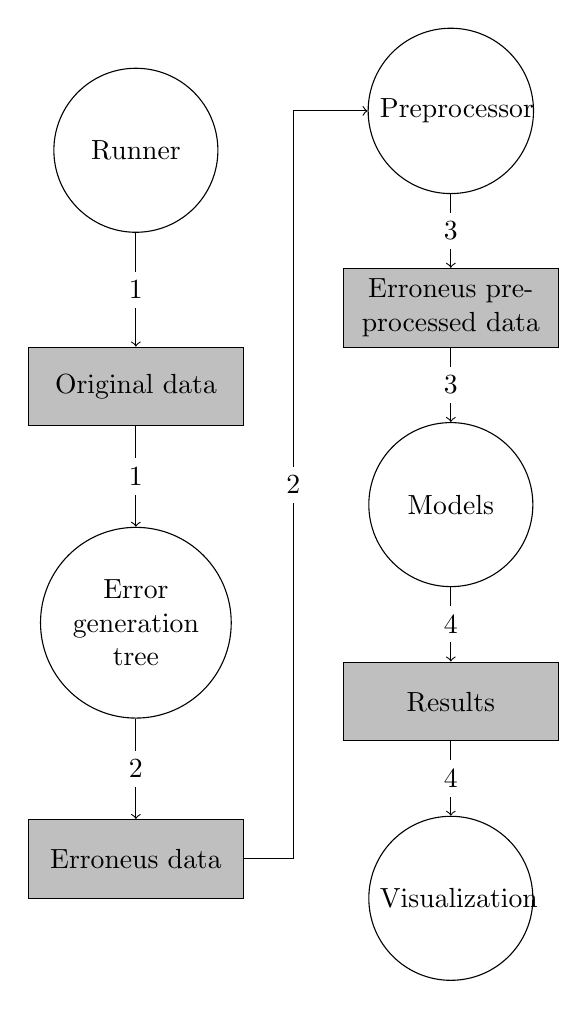
\begin{tikzpicture}[state/.style={circle, draw, align=center, minimum size=1cm, text width=1.8cm},file/.style={rectangle, fill=lightgray, draw, align=center, minimum size=1cm, text width=2.5cm}]
	% nodes

	\node[state] (runner) {Runner};
	\node[file, below of=runner, yshift=-2cm] (origdat) {Original data}; %
	\node[state, below of=origdat, yshift=-2cm] (errtree) {Error generation tree}; %
	\node[file, below of=errtree, yshift=-2cm] (errdat) {Erroneus data}; %
	\node[state, right of=runner, xshift=3cm, yshift=0.5cm] (preproc) {Preprocessor}; %
	\node[file, below of=preproc, yshift=-1.5cm] (eppdat) {Erroneus preprocessed data}; %
	\node[state, below of=eppdat, yshift=-1.5cm] (models) {Models}; %
	\node[file, below of=models, yshift=-1.5cm] (results) {Results}; %
	\node[state, below of=results, yshift=-1.5cm] (visual) {Visualization}; %

	% plate
	% \node[label=above:Data Problems Emulator, draw, inner sep=.5cm, rounded corners=.5cm, fit=(error)(combiner)] (dpemu) {}; %
	% \node[label=below:User Code, draw, inner sep=.5cm, rounded corners=.5cm, fit=(model)(anain)(anlzr)] (user) {}; %

	% edges
	\draw [->] (runner) -- (origdat) node [midway, fill = white] {$1$};
	\draw [->] (origdat) -- (errtree) node [midway, fill = white] {$1$};
	\draw [->] (errtree) -- (errdat) node [midway, fill = white] {$2$};
	\draw [->] (errdat) -- +(2cm, 0) |- (preproc) node [near start, fill = white] {$2$};
	\draw [->] (preproc) -- (eppdat) node [midway, fill = white] {$3$};
	\draw [->] (eppdat) -- (models) node [midway, fill = white] {$3$};
	\draw [->] (models) -- (results) node [midway, fill = white] {$4$};
	\draw [->] (results) -- (visual) node [midway, fill = white] {$4$};
\end{tikzpicture}
\end{document}
